%!TEX root = 00_main.tex

\section{Introduction}

% \commentA{would be nice to show the process figure as a teaser above abstract as in the disney paper}
% Looks like the template doesn't allow us to do this easily unfortunately :(

Machine learning methods that leverage large amounts of training data currently perform best for many problems in computer vision, such as object detection, scene recognition, or gaze estimation~\cite{zhou2014learning,girshick2014rich,zhang15_cvpr}.
However, capturing or collecting large-scale training data can be time-consuming
%, especially for new areas of research without pre-existing datasets.
and supervised learning methods additionally require accurate ground truth annotation for each image.
This annotation process can be expensive and tedious, and there is no guarantee that human-provided labels will be correct.
Ground truth annotation is particularly challenging and error-prone for learning tasks that require highly fine-grained and accurate labels, such as tracking facial landmarks for facial expression analysis and gaze estimation, or body joints for pose estimation and activity recognition.

\begin{figure}
    \includegraphics[width=\columnwidth]{teaser}
    \caption{At the core of our method is a dynamic eye-region model that allows us to render large numbers of photorealistic eye images as training data for eye region registration and gaze estimation.}
    \label{fig:teaser}
\end{figure}

% \commentE{The further back I look, rendering RGB training images does go back into the past for pose-estimation at least, though none of it was ``photorealistic''}
To address these problems, researchers have employed \emph{learning-by-synthesis} techniques to generate large amounts training data with computer graphics.
The advantages of this approach are that both data collection and annotation require little human labour and image synthesis can be geared to specific application scenarios.
Perhaps the best known example is by \citet{shotton2013real}, who synthesized a large and varied depth-image dataset for training a real-time pose-estimator.

The eyes and their movements are important for a range of applications including gaze-based human-computer interaction~\cite{majaranta14_apc}, visual behaviour monitoring~\cite{bulling13_chi,bulling11_pami}, and -- more recently -- computer vision tasks, such as object recognition and detection~\cite{yun2013studying,papadopoulos2014training,karthikeyan2013and}.
The eye-region is particularly difficult to model accurately given the dynamic shape changes it undergoes with facial motion and eyeball rotation, and the complex material structure of the eyeball itself.
For this reason, a recent learning-by-synthesis work for gaze estimation employed only fundamental computer graphics techniques -- rendering low-resolution meshes without allowing lighting variation or accounting for the varying material properties of the face \citet{sugano2014learning}.
In addition, their model was not fully controllable and the synthesized dataset contained only gaze labels, limiting its usefulness for other computer vision problems, such as facial landmark registration.
\commentA{what about Leszeks work? should also fit in here, right?}

% \commentA{we can also remove these last references if we have to save space}
% Recent work by \citet{sugano2014learning} demonstrated the benefits of learning-by-synthesis for appearance-based gaze estimation, but employed only fundamental computer graphics techniques for synthesising low-resolution meshes that did not account for lighting variation.

% It is for this reason that previous work on rendering photorealistic images of the eye and eye-region is relatively sparse~\cite{ActiBlizEyes,berard2014highquality}.
% \commentY{What does this "sparsity" mean? And again, I think having 10 different models is a little to weak to say that it can handle "significant variation in facial shape and texture across different people" in the context of face/eye research.}

% \commentA{we also need to motivate why high quality renderings are needed, i.e. why it's worthwhile to put so much effort into the model. And later we can hopefully also show that it pays off to do so...}

% Andreas: we need some transition to eyeballs here, e.g. eyeball rendering is particularly challenging and interesting because of the many muscles involved, the large number of appearance details around and in the eye etc.
% essentially motivate that this hasn't been done before and is a very interesting area of research

%Synthesising training data is not novel in itself -- previous work has ... Our novel approach 

\begin{figure*}
    \centering
    \begin{subfigure}[t]{0.195\textwidth}
        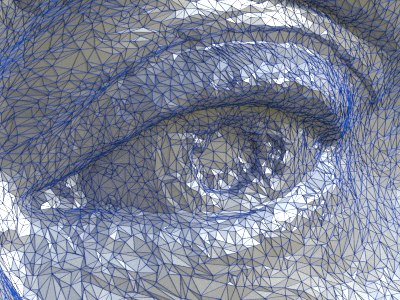
\includegraphics[width=\textwidth]{process_f02_01}
        \caption{Original 3D head scan data: 1.4 million polys}
        \label{fig:process_original_scan}
    \end{subfigure}
    \hfill
    \begin{subfigure}[t]{0.195\textwidth}
        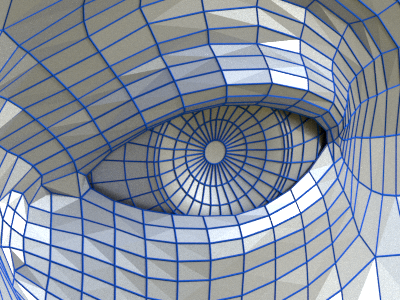
\includegraphics[width=\textwidth]{process_f02_02}
        \caption{Retopologized head model: 9 thousand polys}
        \label{fig:process_retopo}
    \end{subfigure}
    \hfill
    \begin{subfigure}[t]{0.195\textwidth}
        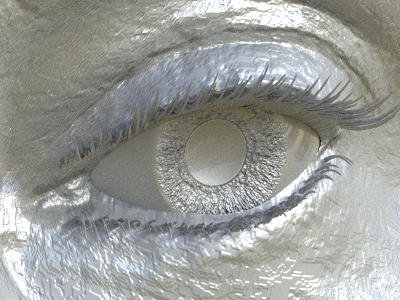
\includegraphics[width=\textwidth]{process_f02_03}
        \caption{Surface detail is stored in displacement maps}
        \label{fig:process_displaced_subdiv}
    \end{subfigure}
    \hfill
    \begin{subfigure}[t]{0.195\textwidth}
        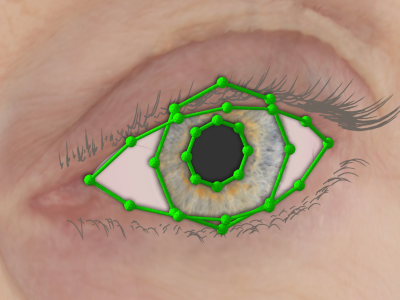
\includegraphics[width=\textwidth]{process_f02_04}
        \caption{3D iris and eyelid landmarks are annotated}
    \end{subfigure}
    \hfill
    \begin{subfigure}[t]{0.195\textwidth}
        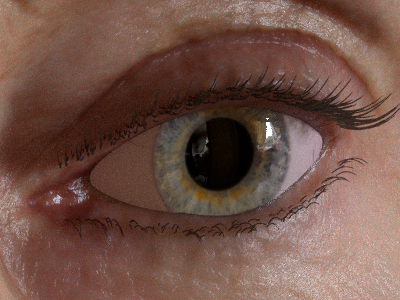
\includegraphics[width=\textwidth]{process_f02_05}
        \caption{The final render}
    \end{subfigure}
    \caption{Model preparation process}
    \label{fig:process}
\end{figure*}

We present a novel method for photorealistic rendering face and eye images at a large scale using a collection of dynamic and controllable eye-region models.
In contrast to previous works, we provide a comprehensive and detailed description of the model preparation process and rendering pipeline (see~\autoref{fig:process} for an overview of the model preparation process and~\autoref{fig:eye_model} for the eye model used).
We then present and evaluate two separate systems trained on the resulting data (\emph{\dataset}): a novel eye-region specific deformable model and an appearance-based gaze estimator.
These systems are case studies that show how we leverage the controllability made available by rendering our training data to easily and quickly generate high quality training datasets.

The specific contributions of this work are threefold.
First, we present our dynamic eye-region model that uses multiple parts and blend shapes to model the continuous degrees of shape change and deformation exhibited by the eye.
We further describe in detail our novel but straight-forward techniques for generating large degrees of realistic lighting variation in synthesized training data using image-based-lighting.
We show that \commentA{insert key gaze estimation result here}
We finally present eye-region registration as a novel application of learning-by-synthesis and demonstrate that \commentA{insert key result here}